\documentclass[aps,prd,reprint,floatfix,nofootinbib,longbibliography]{revtex4-2}
\usepackage[T1]{fontenc}
\input{glyphtounicode}
\pdfgentounicode=1
\usepackage{amsmath,amssymb,bm,graphicx,booktabs}
\usepackage[hidelinks]{hyperref}
\hypersetup{pdfauthor={Abdul Badran},pdftitle={Curvature-matched localized Ricci fluctuations in a prepared Schwarzschild interior}}
\newcommand{\dd}{\mathrm{d}}
\newcommand{\Tr}{\mathcal{T}}
\newcommand{\Pp}{\mathcal{P}}
\newcommand{\Var}{\operatorname{Var}}
\newcommand{\Cov}{\operatorname{Cov}}
\newcommand{\ee}{\epsilon}
\newcommand{\RMS}{\operatorname{SD}}
\newcommand{\Lc}{L_{\!K}}
\begin{document}
\title{Curvature-matched localized Ricci fluctuations in a prepared Schwarzschild interior}
\author{Abdul Badran}
\thanks{Manuscript revision, 28 September 2026. Not peer reviewed.}
\affiliation{Independent Researcher, Texas, USA}
\date{28 September 2026}
\begin{abstract}
We report a reproducible numerical study of finite-resolution, matter-induced curvature fluctuations in a specified prepared state of a real, free, massless, minimally coupled scalar field on a fixed four-dimensional Schwarzschild interior. Proper-time, longitudinal, and angular sampling lengths are matched to fixed fractions of the local curvature length at areal radii $r/M=0.60,0.45,0.30$. A joint pair-amplitude calculation retains the covariance between the stress trace and the squared field time derivative. At leading Einstein order these give the Ricci-scalar and observer-direction Ricci fluctuations without imposing spherical symmetry on the gravitational perturbation. Smooth angular heat kernels are compared with a whole-sphere control and a separately calculated frozen-product vacuum reference. For the narrower localized family and a common illustrative coupling $G\hbar/M^2=10^{-9}$, the Ricci-scalar standard deviation divided by the sampled nonzero background curvature scale increases from $3.5606\times10^{-6}$ to $2.8285\times10^{-5}$. The factor $7.944$ increase is close to the dimensional $r^{-3}$ expectation for curvature-matched sampling. Both primary source standard deviations differ from the matched reference by less than $0.180\%$. Final tested cutoff/refinement changes in the primary variances are below $0.00254\%$, while a deliberately coarse pilot is rejected. These results characterize a state- and resolution-dependent finite-region effect; they do not establish a controlled quantum-dominated regime, a complete fluctuating metric, or a singularity endpoint.
\end{abstract}
\maketitle
\raggedbottom

\section{Introduction and question}
Quantum matter can affect a gravitational description through its mean stress and through connected stress correlations. Semiclassical gravity and stochastic gravity organize these two types of information differently \cite{HuVerdaguer2008,PhillipsHu2001}. A calculation of a nonzero quantum contribution is therefore not, by itself, a test that quantum dynamics has displaced a classical geometric approximation. The relevant questions include the quantity being measured, its resolution, its size relative to a nonzero classical scale, and the domain in which the approximation is controlled.

The motivating question of this project is whether quantum physics becomes essential in the regime that classical relativity describes as a black-hole singularity. No outward pressure, bounce, singularity removal, or Hawking origin of the stress is imposed as a premise. Here we address only one finite-region descendant of that question: do selected localized curvature fluctuations increase relative to a classical curvature scale when all chosen sampling lengths are matched inward? The answer is obtained for one explicit field and prepared state, not for a general quantum theory of the central structure.

Large stress fluctuations relative to a small mean do not alone demonstrate failure of semiclassical gravity \cite{HuPhillips2000}. Stability-based criteria instead involve the response of the geometry and, in general, intrinsic as well as matter-induced metric fluctuations \cite{Anderson2003,HuRouraVerdaguer2004}. The present calculation does not implement those full criteria. It evaluates two local, linearly gauge-invariant Ricci projections using the leading Einstein relations, and distinguishes their numerical and scale checks from a theorem of semiclassical validity.

The noise kernel and its properties are established subjects \cite{PhillipsHu2001}. In particular, approximate Schwarzschild noise calculations already exist for conformally invariant scalar fields in thermal states \cite{Eftekharzadeh2012}. The present state is neither that thermal state nor an Unruh state, and the scalar is minimally rather than conformally coupled. The calculation uses unequal-time mode evolution, normalized spacetime filters, and exact magnetic-index sums for finite angular localization. These differences specify the computational case studied; they are not a claim that stress covariance, angular harmonic reduction, or induced Ricci fluctuations are newly invented concepts.

This paper consolidates the saved numerical release in Ref.~\cite{NumericalArchive}. Its contribution is a defined computational experiment, a joint covariance implementation, matched reference and resolution controls, and a reproducible account of accepted and rejected numerical settings. Earlier mean-backreaction, mass-increment, and normalized tidal-change studies in the project supply historical motivation, not interchangeable numerical evidence. Only the localized inward dataset is used for the numerical tables below. Supplemental Material~\cite{SupplementalMaterial} gives the exact preparation, all result rows, test definitions, provenance, and reproduction instructions.

\section{Geometry, field, and prepared state}
\subsection{Reference geometry and dimensions}
We use signature $(-,+,+,+)$ and set $c=1$. Let $M=G M_{\rm phys}$ denote the geometric mass. Numerical coordinates and mode momenta are measured in units of $M$; thus $M=1$ in the code. On the final measurement region,
\begin{align}
 \dd s^2&=A(\eta)(-\dd\eta^2+\dd x^2)+r(\eta)^2\dd\Omega^2,\label{eq:metric}\\
 A&=2M/r-1,\qquad \frac{\dd r}{\dd\eta}=-A,\qquad 0<r<2M.
\end{align}
Here $\eta$ is timelike and $x$ is the homogeneous longitudinal coordinate. The background is the original Schwarzschild solution, not an extrapolation of a previously corrected mean geometry. Its Kretschmann scalar and the curvature length used to specify sampling are
\begin{equation}
 K_0=\frac{48M^2}{r^6},\qquad \Lc=K_0^{-1/4}.
 \label{eq:curv}
\end{equation}
The timelike sampling direction is $u^a=A^{-1/2}(\partial_\eta)^a$. The metric is spherically symmetric, but the angularly localized test functions below are not uniform over a sphere.

The final field action is
\begin{equation}
 S_\phi=-\frac12\int\dd^4x\sqrt{-g}\,g^{ab}\nabla_a\phi\nabla_b\phi.
 \label{eq:action}
\end{equation}
The field is free, real, massless, and minimally coupled in the region of observation. A smooth auxiliary mass and auxiliary geometry are used only to specify its state. They are not assumed to satisfy the semiclassical Einstein equation or to describe a collapsing star.

\subsection{State prescription and mode normalization}
The state, denoted SPV-1 in the numerical record, is the vacuum obtained by evolving the ground-state modes of an ultrastatic massive past through a specified smooth transition. The dimensionless transition time is $0\leq\eta\leq2$ and the geometry becomes Schwarzschild at $r/M=1.5$. The auxiliary mass-squared begins at $M^{-2}$ and vanishes smoothly. The switching function, initial radius, and differential equations are written explicitly in Supplemental Sec.~S1 and implemented in \texttt{prepared\_geometry.py}. This fixes a mathematical in-state; it does not identify an astrophysical collapse vacuum.

With harmonics normalized by $\int\dd\Omega\,Y_{\ell m}^*Y_{p n}=\delta_{\ell p}\delta_{mn}$, write
\begin{equation}
 \phi=\sum_{\ell m}\int_{-\infty}^{\infty}\frac{\dd k}{\sqrt{2\pi}}
 \left[a_{k\ell m} f_{\ell k}(\eta)e^{ikx}Y_{\ell m}(\Omega)+\mathrm{h.c.}\right],
 \label{eq:field}
\end{equation}
where $[a_{k\ell m},a_{k'pn}^\dagger]=\delta(k-k')\delta_{\ell p}\delta_{mn}$. In numerical units $\hbar=1$; it is restored in the reported variances. Setting $\chi_{\ell k}=r f_{\ell k}$ gives
\begin{equation}
 \chi_{\ell k}''+\left[k^2+A\left(\frac{\ell(\ell+1)}{r^2}+m_{\rm aux}^2\right)-\frac{r''}{r}\right]\chi_{\ell k}=0,
 \label{eq:mode}
\end{equation}
with $\chi\chi^{*\prime}-\chi'\chi^*=i$. The initial modes are positive-frequency ground-state modes in the ultrastatic past. Production evolves a real width/phase representation; separate complex-mode integration is used for representative checks. No absolute renormalized mean-stress table is needed to generate the covariance in this work.

Smooth preparation from a regular massive ground state is the intended ultraviolet state prescription. The present numerical release tests normalization and convergence but does not supply a standalone microlocal proof for its interpolated implementation. Consequently, finite-cutoff numerical checks are not treated as a proof of every Hadamard property. The usual local Wick-observable framework supplies the appropriate setting for renormalized composite operators \cite{HollandsWald2001}.

\section{Finite-resolution observables}
\subsection{Local operators and connected covariance}
Let $\pi=u^a\nabla_a\phi$, and let $|\nabla_\perp\phi|^2$ include the spatial longitudinal and angular derivatives in the background orthonormal frame. The three operators of interest are
\begin{equation}
 \Tr=\pi^2-|\nabla_\perp\phi|^2,\qquad
 \Pp=\pi^2,\qquad \rho=\Pp-\frac12\Tr.
 \label{eq:operators}
\end{equation}
For the minimally coupled massless field, $\Tr=T^a{}_a$ and $\rho=T_{ab}u^a u^b$, up to local identity-valued renormalization terms. The quadratic operator is formed before it is averaged; this is not the square of an averaged linear field.

For a specified common filter, let $Q_A$ be the averaged operator and $\Delta Q_A=Q_A-\langle Q_A\rangle$. The real covariance is
\begin{equation}
 C_{AB}=\frac12\left\langle\Delta Q_A\Delta Q_B+\Delta Q_B\Delta Q_A\right\rangle,
 \quad A,B\in\{\Tr,\Pp\}.
 \label{eq:covariance}
\end{equation}
The supplementary energy variance uses the same matrix,
\begin{equation}
 \Var(Q_\rho)=C_{\Pp\Pp}+\frac14 C_{\Tr\Tr}-C_{\Tr\Pp}.
 \label{eq:rho}
\end{equation}
It is not obtained by adding independent energy and pressure variances. This combination can be much smaller than the parent entries and is therefore a numerically cancellation-sensitive observable.

Adding a fixed local multiple of the identity to a renormalized mean operator leaves $\Delta Q_A$ unchanged. This elementary invariance does not license a divergent pointwise product, settle contact-term questions for every composite observable, or remove the requirement of a specified state and smearing. The connected-noise framework and covariant renormalization issues are distinct from deleting the vacuum contribution \cite{PhillipsHu2001,DecaniniFolacci2008}. In this calculation finiteness is approached through positive pair norms of the explicitly sampled operators and tested spectral extensions.

\subsection{Time, longitudinal, and angular filters}
The averaged observable is
\begin{equation}
 Q_A=\int\dd\tau\,F_\sigma(\tau)
      \int\dd x\,G_{b_x}(x)
      \int\dd\Omega\,H_\delta(\Omega)\,\mathcal O_A(\tau,x,\Omega),
 \label{eq:smearing}
\end{equation}
Here $\mathcal O_A$ denotes the selected local operator. All three filters are normalized. The proper-time kernel is proportional to $e^{-(\tau/\sigma)^2}$, with a smooth compact taper equal to one through $|\tau|=4\sigma$ and zero at $5\sigma$. The proper-time origin is at the chosen central radius. Its exact definition is in Supplemental Sec.~S2.

The longitudinal filter is
\begin{equation}
 G_{b_x}(x)=\frac{e^{-x^2/b_x^2}}{\sqrt{\pi}b_x},\qquad
 b_x=\frac{b_c}{\sqrt{A_c}}.
 \label{eq:longitudinal}
\end{equation}
Thus $b_c$ is the proper exponent width at the center, not at every time in the support. It is not a standard deviation. The proper width evolves as $b_x\sqrt{A(\tau)}$. This distinction is retained in the scale screens.

The angular weight centered at a chosen pole is the positive spherical heat kernel
\begin{equation}
 H_\delta(\theta)=\sum_{J=0}^{\infty}\frac{2J+1}{4\pi}
       e^{-\delta^2J(J+1)/2}P_J(\cos\theta).
 \label{eq:heat}
\end{equation}
It has global tails; it is not a hard cap. The uniform control is $H=1/(4\pi)$ and retains only $J=0$. It is not the limit $\delta\to0$, which localizes rather than averages. The effective angular area fraction is
\begin{equation}
 f_{\rm eff}=\left[\sum_{J=0}^{\infty}(2J+1)e^{-\delta^2J(J+1)}\right]^{-1}.
 \label{eq:area}
\end{equation}
Equation~\eqref{eq:smearing} can be written with the invariant spacetime volume by dividing the scalar test weight by $\sqrt{A}r^2$. This makes clear that it is a specified spacetime observable. It is not a point detector or an assertion of independent random cells.

\subsection{Curvature-matched inward families}
At $x_c=r_c/M\in\{0.60,0.45,0.30\}$, set
\begin{align}
 s_c&=(x_c/0.60)^{3/2}, &\sigma/M&=0.02s_c,\nonumber\\
 b_c/M&=0.25s_c, &\delta&=\delta_0\sqrt{x_c/0.60},
 \label{eq:scales}
\end{align}
with $\delta_0=0.25$ and $0.50$. Then $\sigma$, $b_c$, and $r_c\delta$ are fixed fractions of $\Lc(r_c)$. They do not make the full geometry, directional expansion rates, or every point in a finite window identical. A whole-sphere control is retained but is not itself a curvature-matched local angular patch.

Table~\ref{tab:sampling} collects the sampling parameters and full time-support intervals.

\begin{table}[tb]
\caption{Primary sampling families. Radii and lengths are in units of $M$. The last column is the entire compact time support expressed as an areal-radius interval, not only its quadrature nodes. The wider angular family has twice the listed $\delta$.}
\label{tab:sampling}
\begin{ruledtabular}
\begin{tabular}{ccccc}
$x_c$&$\sigma/M$&$b_c/M$&$\delta_{\rm narrow}$&$r/M$ support\\
0.60&0.020000&0.250000&0.250000&[0.430227,0.740781]\\
0.45&0.012990&0.162380&0.216506&[0.316538,0.561633]\\
0.30&0.007071&0.088388&0.176777&[0.207128,0.378262]
\end{tabular}
\end{ruledtabular}
\end{table}
All supports lie above the retained analytic field-domain boundary $r/M=0.2$. The centers are deep inside the horizon but are not arbitrarily close to $r=0$. No early-to-late difference kernel is used here, unlike the separate mass-increment and normalized tidal-change studies in the project.

\section{Pair-amplitude computation and reference}
\subsection{Angular reduction and the joint matrix}
In a Gaussian vacuum, Wick contraction reduces Eq.~\eqref{eq:covariance} to a two-particle norm. Define $d_{\ell k}=f'_{\ell k}$ and, for two angular orders $\ell,p$ and two positive momenta $k,k'$, the time-integrated matrices
\begin{align}
 D_{\ell p}&=\int\dd\tau F_\sigma\frac{d_{\ell k}d_{pk'}}{A},\nonumber\\
 X_{\ell p}&=\int\dd\tau F_\sigma\frac{f_{\ell k}f_{pk'}}{A},\nonumber\\
 Z_{\ell p}&=\int\dd\tau F_\sigma\frac{f_{\ell k}f_{pk'}}{r^2}.
 \label{eq:matrices}
\end{align}
There is no complex conjugation inside an $aa$ amplitude. Conjugation enters when taking its norm. For the two relative momentum signs $s=\pm1$,
\begin{equation}
 B_J^{(s)}=D+s kk'X-\frac{\ell(\ell+1)+p(p+1)-J(J+1)}{2}Z.
 \label{eq:B}
\end{equation}
The source-amplitude vector is $v_J^{(s)}=(B_J^{(s)},D)^T$. The energy amplitude is $D-B_J^{(s)}/2$.

Using the Gaunt identity and magnetic-index orthogonality \cite{DLMF}, the covariance spectrum in the conventions of Eq.~\eqref{eq:field} is
\begin{align}
 \mathcal G_{\ell pJ}&=\frac{(2\ell+1)(2p+1)(2J+1)}{16\pi^4}
 \begin{pmatrix}\ell&p&J\\0&0&0\end{pmatrix}^{\!2},\nonumber\\
 S_{AB}^{J}&=\sum_{\ell\leq p}(2-\delta_{\ell p})\mathcal G_{\ell pJ}
 \int_0^{\infty}\dd k\int_0^{\infty}\dd k'\nonumber\\
 &\quad\times\sum_{s=\pm1}e^{-b_x^2(k+s k')^2/2}
 \operatorname{Re}[v_{J,A}^{(s)}v_{J,B}^{(s)*}],\label{eq:spectrum}\\
 C_{AB}(\delta)&=\sum_J e^{-\delta^2J(J+1)}S_{AB}^{J}.
 \label{eq:angularcov}
\end{align}
Triangle and even-parity conditions are imposed. The factor of two from the vacuum two-particle norm, momentum-sign reduction, and unequal-angular-order multiplicity are included. The uniform case selects $S^0$. Thus averaging the gravitational observable over a sphere does not mean retaining only scalar field modes with $\ell=0$.

Each angular pair stores six real moments from which the entire $2\times2$ spectrum can be rebuilt for every retained $J$. Positive pair norms establish the expected covariance positivity; independent angular, mode-phase, and direct-pair checks test the implementation. No covariance element or pressure is adjusted to impose an identity.

\subsection{Frozen-product control}
The independent reference freezes $r$ and $A$ at the central values and uses a massless positive-frequency state on the resulting ultrastatic product geometry. Its mode frequencies are
\begin{equation}
 \omega_{\ell k}^{\rm fr}=\sqrt{k^2+A_c\ell(\ell+1)/r_c^2}.
\end{equation}
The same proper-time, longitudinal, and angular filters are applied. Products in Eq.~\eqref{eq:matrices} are replaced by their analytic frequency representation, including
\begin{equation}
 f_\ell f_p\longmapsto
 \frac{\widehat F_\sigma[(\omega_\ell+\omega_p)/\sqrt{A_c}]}{2r_c^2\sqrt{\omega_\ell\omega_p}},
 \label{eq:frozen}
\end{equation}
with $D=-\omega_\ell\omega_p f_\ell f_p/A_c$. The compact-kernel transform is evaluated with a separately checked interpolation against direct quadrature.

This is a derivative-stress comparison, not an Einstein solution on the frozen product and not the same global state or history as the interior. The massless undifferentiated zero-mode infrared issue is not claimed to be resolved for general $\phi^2$; the calculation concerns derivative observables. Agreement with the reference is not an exact partition of the measured noise into independent static and dynamical contributions. In particular, variances from these two different models should not be subtracted as though they were independent random sources.

\section{Leading gravitational interpretation}
At leading Einstein order on the Ricci-flat background,
\begin{align}
 \delta R&=-8\pi G\,\Delta\Tr,\nonumber\\
 \delta(R_{ab}u^a u^b)&=8\pi G\,\Delta\Pp,\label{eq:ricci}\\
 \delta(G_{ab}u^a u^b)&=8\pi G\,\Delta\rho.\nonumber
\end{align}
Here $\Delta$ refers to the centered source. These are the necessary local projections of a matter-induced perturbation; they are not a reconstruction of its complete metric. Since the reference Ricci tensor is zero, its first perturbation and these specified background-frame projections are linearly gauge invariant. Frame changes multiplying the background Ricci tensor do not contribute at this order. This does not remove gauge and constraint questions for a full Weyl or metric response.

The source cross entry $C_{\Tr\Pp}$ is not the Ricci cross entry. The latter is obtained by multiplying the source matrix on both sides by $(8\pi G)\operatorname{diag}(-1,1)$. The energy combination is an Einstein-tensor projection, not an additional Ricci eigenvalue.

For gravitational magnitude we use a nonzero background scale,
\begin{equation}
 D_c=\int\dd\tau F_\sigma(\tau)\frac{\sqrt{48}}{[r(\tau)/M]^3},
 \qquad \ee=\frac{G\hbar}{M^2},
\end{equation}
so that, for the appropriate numerical variance $V_A$,
\begin{equation}
 \chi_A=\frac{\RMS(\delta\mathcal R_A)}{\langle\sqrt{K_0}\rangle}
       =\ee\frac{8\pi\sqrt{V_A}}{D_c}.
 \label{eq:chi}
\end{equation}
Physical stress standard deviations have units $\hbar/M^4$, and their variances have units $\hbar^2/M^8$. The denominator is neither background Ricci, which vanishes, nor a nearly zero quantum mean. Nevertheless, $\chi_A$ is only one scale comparison. It is not the variance of $K$, a percentage of all gravity, a maximum excursion, or a rare-event probability. Quadratic-field statistics need not be Gaussian; a second moment does not supply the probability distribution \cite{FewsterFordRoman2012}.

\section{Numerical design and validation}
The production record comprises seven campaigns: one coarse pilot and a main/fine pair at each radius. All are separately saved, not inferred from counts in a narrative. In total, 187,904 $(\ell,k)$ labels were evolved and 896 angular contraction blocks stored. The count is not multiplied by harmonic degeneracy or the number of pair contractions. The finest configurations are shown in Table~\ref{tab:grids}; full main and pilot settings are in Supplemental Table~S2.

\begin{table}[tb]
\caption{Finest production settings. $L$ is the largest scalar angular order, $K_{\max}$ the positive longitudinal cutoff, and $n_k,n_\tau$ the quadrature sizes. All retain external harmonics through $J=32$ and use ODE relative tolerance $2\times10^{-11}$.}
\label{tab:grids}
\begin{ruledtabular}
\begin{tabular}{ccrrr}
$r_c/M$&$L$&$K_{\max}M$&$n_k$&$n_\tau$\\
0.60&127&256&192&320\\
0.45&159&480&224&384\\
0.30&191&960&256&448
\end{tabular}
\end{ruledtabular}
\end{table}

No fitted ultraviolet tail is added to the final covariance. Positive-momentum integration uses Gauss--Legendre nodes. Time integration uses the actual compact support and normalized proper-time weights. The ODE implementation uses DOP853 with an absolute tolerance equal to the relative tolerance divided by 100. Exact end states and source/configuration fingerprints are saved per angular order. Approximate, phase-resolved history caches were built afterward and checked separately; they are not inputs replacing the production time integrals.

The declared tests distinguish scalar-field angular cutoff $L$ from external measurement harmonic cutoff $J$. For each output, the fine-grid spectra are restricted to the main $L$ and compared with the unrestricted fine result. The restricted fine result is then compared with the main result; this second comparison changes momentum cutoff, quadrature, time resolution, and solver tolerance jointly. It does not isolate those errors one at a time. The reference is tested in the same manner.

\begin{table}[tb]
\caption{Largest primary-variance changes across the angular filters, expressed as percentages. These are numerical sensitivities, not statistical or physical uncertainty intervals.}
\label{tab:errors}
\begin{ruledtabular}
\begin{tabular}{cccc}
$r_c/M$&Field $L$&Matched-$L$&$J:24\to32$\\
0.60&$6.17\times10^{-6}$&$9.90\times10^{-6}$&$<4\times10^{-14}$\\
0.45&$1.86\times10^{-8}$&$4.13\times10^{-5}$&$1.36\times10^{-11}$\\
0.30&$7.85\times10^{-9}$&$2.538\times10^{-3}$&$2.77\times10^{-7}$
\end{tabular}
\end{ruledtabular}
\end{table}

Table~\ref{tab:errors} summarizes the primary numerical refinement comparisons.

All 43 Boolean entries in the archived final acceptance record are true, including supplementary energy checks, reference checks, overlap, and positive covariance. The representative independent tests include symbolic Wigner coefficients, Gaunt and angular-gradient quadratures, direct versus moment-reduced pairs, independent complex versus width/phase modes, proper-time support, reference Fourier integration, phase invariance, and trace reversal. These tests do not amount to a complete position-space Ward-identity audit of every component of a tensor noise kernel.

The pilot differs from the finest results by as much as $30.48\%$ for a reported variance and is rejected. Its outputs remain available. The smallest normalized eigenvalue of the reported source covariance matrices is approximately $1.50\times10^{-4}$, consistent with positive definiteness while also showing that some linear combinations are much smaller than the parent entries. Further accuracy issues for such combinations must be assessed with conditioned rather than solely entrywise relative norms.

A separate manuscript-stage audit verified all 4,169 file hashes in the source release, reduced the 480 fine-grid contraction blocks directly, and reconstructed the 27 result rows. It also reran the bounded independent-check suite in a fresh temporary tree. These are fresh verification and reassembly operations, not a new production field campaign. The primary variance differences from the saved table were below $5.5\times10^{-16}$ relative in the current audit. Supplemental Material documents the cancellation-sensitive supplementary comparison and a different reduction-order check recorded during an earlier interrupted draft. No original numerical arrays were altered.

\section{Results}
\subsection{Localized inward comparison}
Figure~\ref{fig:ratios} displays the two primary curvature comparisons for the narrow angular family.
For the narrow family $\delta_0=0.25$, Table~\ref{tab:primary} gives the two primary source standard deviations, their frozen-reference ratios, and the dimensionless coefficients $\chi_A/\ee$. All normalization factors in Eq.~\eqref{eq:chi} are applied after the covariance calculation.

\begin{table*}[tb]
\caption{Primary narrow-family results. $\RMS(Q)$ is in units $\hbar/M^4$; reference ratios compare source standard deviations, not gravitational dominance. Percentages use the same illustrative $\ee=10^{-9}$ at every radius. Extra digits facilitate replication and do not indicate a total physical error bar.}
\label{tab:primary}
\begin{ruledtabular}
\begin{tabular}{ccccccc}
$r_c/M$&Projection&$\RMS(Q)$&$\RMS(Q)/\RMS(Q_{\rm fr})$&$D_c$&$\chi_A/\ee$&$100\chi_A$\\
0.60&$\delta R$&4586.4380&0.99820350&32.374004&3560.5655&0.00035606\%\\
0.45&$\delta R$&25700.9891&0.99821225&76.803681&8410.2259&0.00084102\%\\
0.30&$\delta R$&291972.0135&0.99822271&259.433293&28284.9474&0.00282849\%\\
0.60&$\delta R_{uu}$&2310.2611&1.00038081&32.374004&1793.5129&0.00017935\%\\
0.45&$\delta R_{uu}$&12947.4773&1.00048331&76.803681&4236.8489&0.00042368\%\\
0.30&$\delta R_{uu}$&147107.5590&1.00060752&259.433293&14251.1247&0.00142511\%
\end{tabular}
\end{ruledtabular}
\end{table*}

The Ricci-scalar comparison grows by $7.94395$ between $r/M=0.60$ and $0.30$. The observer-direction comparison grows similarly. This is an increase relative to the chosen classical curvature scale, not just an increase in an unnormalized stress. It remains a comparison of finite-resolution observables whose physical supports shrink inward.

\begin{figure}[tb]
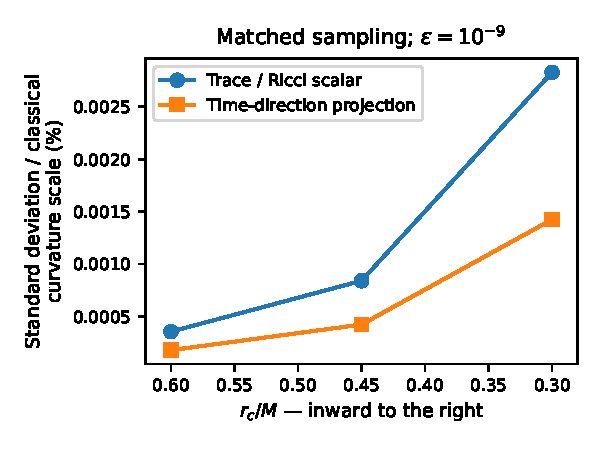
\includegraphics[width=\columnwidth]{figures/curvature_ratios.pdf}
\caption{Primary narrow-family induced-curvature standard deviations relative to the sampled background scale, at a common $\ee=10^{-9}$. The horizontal direction runs inward. Curves connect three computed points and are not an extrapolation toward the singularity.}
\label{fig:ratios}
\end{figure}

The wider angular family and uniform control are also included in Supplemental Table~S1. For example, at $r/M=0.60$ the trace standard deviations for uniform, $\delta=0.50$, and $\delta=0.25$ are approximately $1141.23$, $2377.25$, and $4586.44$. Narrowing the angular weight increases the sampled fluctuation. The effective area of the narrow family decreases from $6.12\%$ to $3.09\%$ of the sphere over the inward comparison, even though its proper diffusion-width convention is matched to curvature. The uniform control should not be confused with that matched local family.

\subsection{What the reference does and does not explain}
Figure~\ref{fig:reference} displays the departures of the two primary source standard deviations from their matched reference values.
Across all nine primary windows, the trace/reference standard-deviation ratio lies between $0.9982035$ and $0.9982291$; the corresponding time-projection ratio is between $1.0003754$ and $1.0006075$. Both are within $0.180\%$ of unity. This agreement indicates that a substantial part of the observed primary behavior is already accounted for by the reference with matched filters. It does not identify the residual as an isolated new physical contribution, nor show that preparation and geometry are individually negligible.

\begin{figure}[tb]
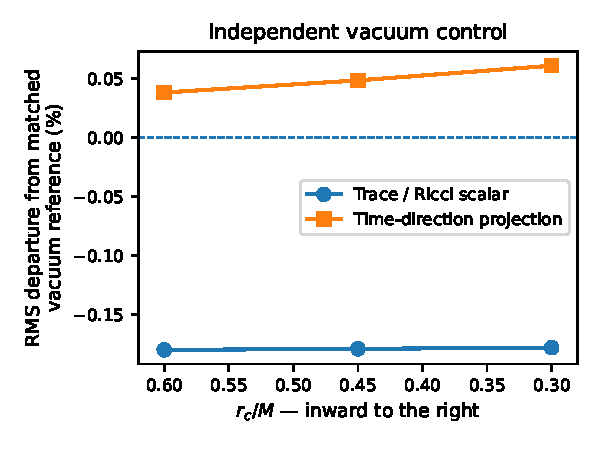
\includegraphics[width=\columnwidth]{figures/reference_offsets.pdf}
\caption{Narrow-family fractional RMS departures from the independently calculated frozen-product reference. No coefficients are fitted to the interior data. The comparison is local to the specified operators and filters, not an equality of full geometries or states.}
\label{fig:reference}
\end{figure}

The reference result is itself quantum. Agreement with it therefore does not make the measured fluctuation classical, and does not logically rule out quantum importance at other scales. A residual-to-reference ratio and a ratio to classical curvature answer different questions. The former tests a comparison model; the latter assesses one gravitational magnitude at the chosen coupling.

\subsection{Supplementary energy combination}
The energy combination of Eq.~\eqref{eq:rho} is retained as a secondary diagnostic. In the narrow family its source/reference RMS ratios are $2.736$, $2.872$, and $3.032$ inward. Its standard deviations are only about $74.93$, $441.93$, and $5315.17$ in the same field units, much smaller than the primary trace values. Their gravitational percentages at $\ee=10^{-9}$ are approximately $0.00000582\%$, $0.00001446\%$, and $0.00005149\%$.

This is a difference of strongly correlated terms. Its larger ratio to a small reference is not a larger ratio to classical gravity. It cannot be interpreted as a new independent noise source. No additional prepared-state sweep was performed in the localized inward release, and the earlier project's prepared-state controls involve different observables. Their insensitivity is not transferred to the present energy diagnostic.

\section{Validity, interpretation, and limitations}
\subsection{A conditional dimensional control}
There is a useful dimensional interpretation of the inward trend. If short-distance stress fluctuations scale approximately as the inverse fourth power of a common sampling length, and all local lengths are proportional to $\Lc$, then
\begin{equation}
 \RMS(Q)\sim\hbar\Lc^{-4},\qquad
 \chi\sim G\hbar\Lc^{-2}\propto r_c^{-3}.
 \label{eq:dimensional}
\end{equation}
The associated factor from $0.60M$ to $0.30M$ is eight. The actual narrow-family trace factor is $7.94395$, corresponding to a two-point descriptive exponent $2.9899$. This is a manuscript-stage dimensional control and arithmetic summary, not a newly simulated mechanism or a fitted universal law. Finite sphere curvature, anisotropic evolution, the state, and noninfinitesimal filters prevent exact self-similarity. The reference calculation, rather than dimensional reasoning alone, provides the quantitative comparison.

\subsection{Scale separation is not a validity theorem}
At a fixed numerical configuration Eq.~\eqref{eq:chi} is linear in $\ee$. Changing $\ee$ algebraically is not a new field evolution. The illustrative $10^{-9}$ value gives temporal exponent widths of approximately $632$, $411$, and $224$ Planck times for the three centers. Widths are conventions of smooth filters, not physical ultraviolet cutoffs.

The release also defines conditional screens using the minimum of the time width, the longitudinal proper width over the support, the angular diffusion width over the support where present, the minimum radius, and the minimum curvature length. Requiring this minimum to exceed $N\ell_P$ gives
\begin{equation}
 \ee\leq(\lambda_{\min}/N)^2,
 \label{eq:screen}
\end{equation}
where $\lambda_{\min}$ is dimensionless in units $M$. For $N=10,30,100$, the largest allowed percentage among the tabulated projections is respectively $1.4242\%$, $0.15825\%$, and $0.014242\%$. These are per-window maxima under chosen screening rules, not the radial history of one black hole with changing coupling.

No $N$ here is an experimentally established transition or a sufficient effective-field-theory bound. The screens omit full polarization, all local higher-curvature response, intrinsic metric fluctuations, and other field content. Setting the extrapolated primary ratio to unity would place temporal widths at approximately $0.35$--$1.19$ Planck times. That is outside the scale-separated claim being made. It is not a numerical location of quantum takeover or a solution of the singularity.

\subsection{Field and gravitational scope}
The scalar curvature coupling matters. For a massless conformally invariant scalar field the trace of the noise kernel vanishes, despite a possible identity-valued mean trace anomaly \cite{PhillipsHu2001}. Thus a trace-based result for minimal coupling cannot represent all quantum matter. The time-direction Ricci source must also be rederived when the stress tensor is improved; it is not legitimate simply to reuse $\Pp=\pi^2$ for every coupling.

The most immediate additional control is therefore an improved-stress calculation at fixed final Ricci-flat geometry and fixed final Cauchy state, comparing minimal and conformal coupling while retaining a nontrace observable. A separate calculation may vary the preparation consistently with the coupling: its auxiliary geometry is not generally Ricci flat, so those two experiments are different. No such coupling sweep is reported here.

The Ricci projections in Eq.~\eqref{eq:ricci} do not provide localized Weyl or tidal covariance, the retarded metric propagator, gravitational initial data, or an Einstein--Langevin solution. The distinction between induced and intrinsic fluctuations must be retained in a fuller calculation \cite{HuRouraVerdaguer2004}. A later nonspherical response study must propagate conserved source correlations with specified initial and boundary data, rather than insert unrelated random energy kicks into homogeneous mean equations.

Other restrictions are substantive: one Gaussian prepared state, no physical collapse construction, no electromagnetic or spinor fields, no interactions, a fixed nonrotating background, three locations, smooth global angular and longitudinal tails, and no final-state geometry response in the fluctuation calculation. The numerically small changes in cutoff tests do not bound these physical approximations. Numerical convergence, field-state admissibility, gravitational approximation validity, and novelty are separate questions.

\section{Conclusions}
A joint covariance of two quadratic scalar-field observables was calculated on three curvature-matched, angularly localized windows in a prepared Schwarzschild interior. The leading Einstein relations assign these covariances a limited Ricci-curvature interpretation without applying spherical mass or Weyl identities to a nonspherical patch. Full trace/time cross correlations are retained, and a supplementary energy combination is evaluated from the same pairs.

For the narrow localized family, the Ricci-scalar standard deviation relative to a nonzero sampled background curvature scale increases by a factor $7.944$ when the central radius halves. At a common illustrative $\ee=10^{-9}$ the ratio remains below $2.83\times10^{-5}$. The primary source standard deviations agree with their separately calculated frozen-product controls within $0.180\%$. The growth is therefore not, on its own, evidence for an unexplained singularity-specific mechanism. Agreement with an ordinary quantum reference also does not prove quantum effects can never become important; the magnitude and validity questions remain separate.

The finite-region result supports neither a universal quantum-dominance claim nor a universal exclusion of it. It supplies a reproducible numerical test and a restriction on how growth of sampled fluctuations may be interpreted. A field-coupling/nontrace control and a specified causal nonspherical gravitational observable are more discriminating next steps than repeatedly narrowing the same windows. Quantum coherence of a rotating central ring, singularity hit/bypass probabilities, and a cosmological-origin analogy are outside the present model.

\section*{Competing interests}
The author declares no competing interests.

\section*{Funding}
This research received no external funding.

\section*{Ethical approval}
Not applicable. This is a theoretical and computational physics study involving no human participants, human research data, animals, or biological materials. Ethical approval was not required.

\section*{Data availability}
The data and software supporting this study are available upon reasonable request from the author. They are preserved in the computational reproducibility record identified in Ref.~\cite{NumericalArchive}, which contains the source code, configurations, covariance blocks, tabulated results, accepted and rejected numerical checks, and reproduction instructions. The accompanying supplement describes that record. A public repository release is being prepared, but its location has not yet been verified for this revision; no public repository URL or DOI is claimed. Working reviewer access and the corresponding submission-form statement must be finalized before submission.

\section*{Verification scope}
Archive verification and a fresh reduction of saved outputs were completed during manuscript preparation. A bounded independent-check suite was also rerun. The full seven-campaign production calculation was not rerun for the manuscript. All numerical conclusions are conditional on the documented model and validated computational procedures; no independent human specialist review or experimental confirmation is claimed.

\section*{Research provenance and AI assistance}
Abdul Badran supplied the motivating conceptual questions and project direction. Mathematical formulations, code, numerical execution, analysis, and drafting in the computational record were developed with substantial AI assistance; these are not represented as his unaided personal derivations. ChatGPT was used for this manuscript and its source/table checks; the drafting record identifies the manuscript model as GPT-6 Astra Pro. Exact historical model versions for every earlier stage have not been independently authenticated. Instructions required source-grounded claims, preserved failure records, runnable calculations, and explicit limitations. Verification undertaken is specified above and in Supplemental Material. AI tools are not authors. The author must review, revise as needed, and take responsibility for all claims and disclosures before submission. No external submission or independent peer review is asserted by this revision.

\bibliography{references}
\end{document}
